\documentclass[12pt]{article}
\pagestyle{empty}

\newcommand{\ray}[1]{\overrightarrow{#1}}
\renewcommand{\line}[1]{\stackrel{\longleftrightarrow}{#1}}

\renewcommand{\deg}{^{\circ}}
\renewcommand{\parallel}{\mathbin{\|}}
\newcommand{\pr}{^{\prime}}
\newcommand{\ppr}{^{\prime\prime}}
\newcommand{\qd}{\Box}
\newcommand{\seg}[1]{\overline{#1}}

\newcommand{\C}{\cal C}

\newcommand{\forward}{\noindent ($\Longrightarrow$) \,\,}
\newcommand{\back}{\noindent ($\Longleftarrow$) \,\,}
\newcommand{\R}{\mathbb R} %REALS
%\newcommand{\C}{\mathbb C} %COMPLEX
\newcommand{\N}{\mathbb N} %NATURAL NUMBERS
\newcommand{\Q}{\mathbb Q} %RATIONALS
\newcommand{\Z}{\mathbb Z} %INTEGERS
\renewcommand{\o}{\circ}
\newcommand{\Int}[1]{{\cal I}nt( #1)}
\newcommand{\spifff}{\qquad\text{iff}\qquad}
\newcommand{\spand}{\qquad\text{ and }\qquad}
\newcommand{\imp}{\Rightarrow}
\newcommand{\ifff}{\Leftrightarrow}

%\newenvironment{proof}{\smallskip \noindent {\bf Proof:}}{ 

%\smallskip}
\usepackage{amsthm}
\usepackage{amssymb} 
\usepackage{graphicx} 
\usepackage{enumerate}
\usepackage{amsmath} 

\begin{document}
\begin{center}
{\bf Final Celebration of Learning}\\
Euclidean and Non-Euclidean Geometry\\
Sam Chong Tay\\
Fall, 2012
\end{center}


\begin{enumerate}
\item (5 pts) Let $\ell$ be a line and let $A$ and $B$ be distinct points on the same side of $\ell$ such that $d(A, \ell) = d(B, \ell)$.  Suppose that $P$ and $Q$ are the feet of the perpendiculars from $A$ to $\ell$ and from $B$ to $\ell$.  Prove that $\qd PQBA$ is a Saccheri quadrilateral. 
\begin{center}
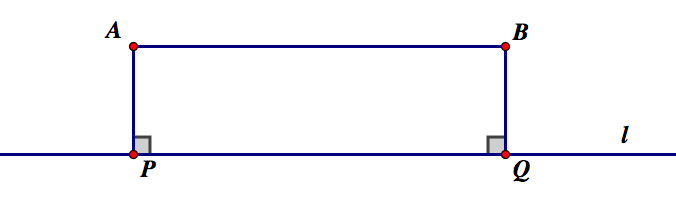
\includegraphics[width=4in]{1a.png}
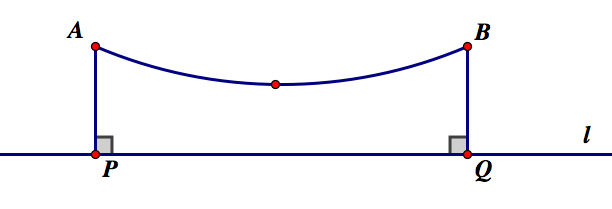
\includegraphics[width=3.8in]{1b.png}

\end{center}

\begin{proof}
First we must show that $\qd PQBA$ is in fact a quadrilateral. This requires proof that no three of the points $P,Q,B,A$ are collinear. Note that since neither $A$ nor $B$ lie on $\ell$, we have $A\ne P$ and $B\ne Q$, so we can refer to the lines $\line{PA}$ and $\line{QB}$. We need to show $P$ and $Q$ are distinct as well; this will follow from the fact that $\line{PA} \ \ne \ \line{QB}$. Because the line $\line{PA}$ perpendicular to $\ell$ through $P$ is unique we see that $P=Q$ implies $\line{PA} \ = \ \line{QB}$, so that $B\in \line{PA}$. Furthermore since $A$ and $B$ are on the same side of $\ell$, it must be the case that $B\in\ray{PA}$. However by hypothesis it follows that $$d=PA=d(A,\ell)=d(B,\ell)=QB=PB,$$ and by Theorem 3.2.23 the point $A$ on $\ray{PA}$ with $PA=d$ is unique. So this would imply $A=B$, contradicting hypothesis; therefore $P\ne Q$. Note the order of this argument also shows that, by contradiction, it must be the case that $\line{PA} \ \ne \ \line{QB}$ and $B\notin \line{PA}$,  and a similar argument shows $A\notin\line{QB}$.

Now that $P$ and $Q$ have been shown to be unique we refer to $\ell$ as $\line{PQ}$. Considering the four ways to pick three distinct points:
\begin{enumerate}[(i)]
\item $A\notin\line{PQ}$ by hypothesis
\item $B\notin\line{PQ}$ by hypothesis
\item $B\notin\line{PA}$ as seen in the argument above
\item $A\notin\line{QB}$ by the same argument above.
\end{enumerate}
Therefore no three of the points $P,Q,B,A$ are collinear. Next we need to show that the segments $\seg{PQ}, \seg{QB}, \seg{BA},$ and $\seg{AP}$ are either disjoint or share at most an endpoint. We have already argued that $\line{PA} \ \ne \ \line{QB}$ and $P\ne Q$, so by definition we have $\line{PQ}$ as a transversal for the lines $\line{PA}$ and $\line{QB}$. Furthermore since $\line{PA}\perp\line{PQ}$ and $\line{QB}\perp\line{PQ},$ it follows from Exercise 3.5.1 that the alternate interior angles must be right angles and are thus congruent. Therefore by the Alternate Interior Angles Theorem, we have $\line{PA} \| \line{QB}$. Certainly then $\seg{PA} \cap \seg{QB} = \emptyset$. Also $\seg{AB} \ \cap \line{PQ} \ = \emptyset$ because $A$ and $B$ are on the same side of $\line{PQ}$, so it is clear that $\seg{AB}\cap\seg{PQ}=\emptyset$. Finally because no three of the points are collinear, we know that the lines $\line{PQ}, \line{QB},\line{BA},$ and $\line{AP}$ are distinct and thus the intersection of any two of them is at most one point. Therefore 
$$\seg{PQ}\cap\seg{QB}=\{Q\}$$
$$\seg{QB}\cap\seg{BA}=\{B\}$$
$$\seg{BA}\cap\seg{AP}=\{A\}$$
$$\seg{AP}\cap\seg{PQ}=\{P\}.$$
We have now shown that any three of $P,Q,B,$ and $A$ are noncollinear and any two of the segments $\seg{PQ}, \seg{QB}, \seg{BA},$ and $\seg{AP}$ are either disjoint or have only an endpoint in common. Therefore $\qd PQBA$ is a quadrilateral.

The fact that this quadrilateral is a Saccheri quadrilateral is immediate: by hypothesis $$AP = d(A,\ell) = d(B, \ell) = BQ,$$ and by construction we know that $$\angle APQ \spand \angle BQP$$ are right angles. Therefore $\qd PQBA$ is a Saccheri quadrilateral with base $\seg{PQ}$.
\end{proof}

\item  (10 pts) Suppose that $A \ast B \ast C$ and that $D$ is an exterior point to line $\line{AB}$.  Let $\ray{BP}$ and $\ray{BQ}$ be the angle bisectors of the angles $\angle ABD$ and $\angle CBD$. Then the rays $\ray{BP}$ and $\ray{BQ}$ form a right angle. 

\begin{proof} Note that since $A \ast B \ast C$, $\ray{BA}$ and $\ray{BC}$ are opposite rays. By definition $\angle ABD$ and $\angle DBC$ form a linear pair and by the Linear Pair Theorem, $$\mu(\angle ABD) + \mu(\angle DBC) = 180^\o.$$ By definition of angle bisectors we have $P$ in the interior of $\angle ABD$ and $Q$ in the interior of $\angle DBC$ such that for some fixed real numbers $x$ and $y$,
$$x^\o=\mu(\angle ABP) + \mu(\angle PBD)$$
$$y^\o=\mu(\angle DBQ) + \mu(\angle QBC).$$
By the Angle Addition Postulate,
\begin{align*} 180^\o &= \mu(\angle ABD) + \mu(\angle DBC)\\
				&=\mu(\angle ABP) + \mu(\angle PBD)+\mu(\angle DBQ) + \mu(\angle QBC)\\
				&=2x^\o + 2y^\o\\
				&=2(x^\o +y^\o).
\end{align*}
\begin{center}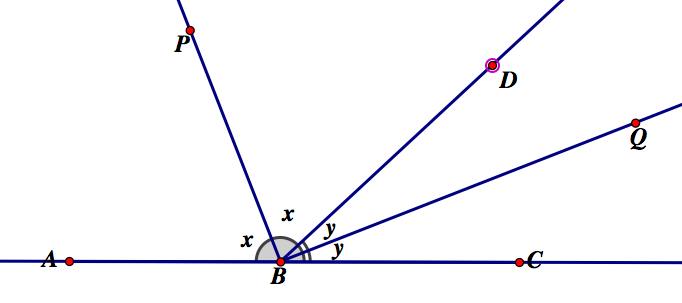
\includegraphics[width=3.8in]{2a.png}\end{center}
Hence $$90^\o=x^\o+y^\o = \mu(\angle PBD) + \mu(\angle DBQ).$$ If we can show that $D$ is in the interior of $\angle PBQ$, we can finish the proof using the Angle Addition Postulate.

First we need to show $\angle PBQ$ exists. To that end note that that if $\ray{BP}$ and $\ray{BQ}$ were opposite rays so that $P\ast B \ast Q$, then since $D\notin\line{BC}$, $\mu(\angle DBC)>0$ and hence $\mu(\angle QBC) = \frac{1}{2}\mu(\angle DBC) >0$ as well, so that $Q\notin\line{BC}$. Then $P\ast B\ast Q$ implies $P$ is on the opposite side of $\line{AB}$ from $Q$ and thus on the opposite side of $\line{AB}$ from $D$. This contradicts $P$ in the interior of $\angle ABD$.
 \begin{center}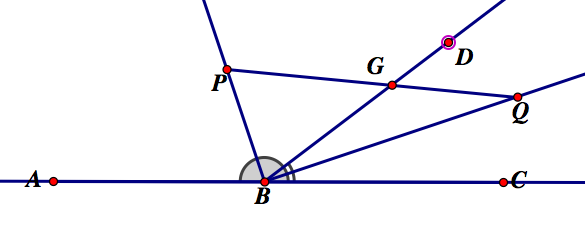
\includegraphics[width=3.8in]{2b.png}\end{center}
 
Because $P$ is in the interior of $\angle ABD$ and $Q$ is in the interior of $\angle DBC$, we have $P$ and $A$ on the same side of $\line{DB}$, and $Q$ and $C$ on the same side of $\line{DB}$. However since $A\ast B\ast C$, we see that $A$ and $C$ are on opposite sides of the line $\line{DB}$ and therefore $P$ and $Q$ are on opposite sides of $\line{DB}$. Hence the line $\line{DB}$ intersects the interior of $\seg{PQ}$ at a point $G$. However, from the fact that $P$ is in the interior of angle $\angle ABD$ and $Q$ is in the interior of angle $\angle DBC$, we also infer that $P,Q,$ and $D$ are all on the same side of line $\line{AB}=\line{BC}$. Thus by convexity of the half-plane, since $G\in\seg{PQ}$ it must be the case that $G$ is on the same side of $\line{AB}$ as $D$ as well. Hence $\seg{PQ}$ intersects the ray $\ray{AD}$ at $G$, and by Theorem 3.5.3 we finally conclude that $D$ is in the interior of angle $\angle PBQ.$ Therefore
\begin{align*} \mu(\angle PBQ) &= \mu(\angle PBD) + \mu(\angle DBQ)\\
						&=x^\o + y^\o\\
						&= 90^\o,
\end{align*}  so $\angle PBQ$ is a right angle.
\end{proof}

\item (5 pts) Prove that a triangle is equilateral if and only if each of its angles measures $60^{\circ}$. 

\begin{proof} \forward Suppose $\triangle ABC$ is an equilateral triangle. Then by SSS we have $$\triangle ABC \cong \triangle BCA \cong \triangle CAB,$$ so $$\angle ABC \cong \angle BCA \cong \angle CAB.$$ By Theorem 5.1.3 we know that $\sigma(\triangle ABC) = 180^\o$, so it must be the case that each angle measures $\frac{180^\o}{3} = 60^\o.$

\back Suppose each angle of triangle $\triangle ABC$ measures $60^\o$. Then since any two of the angles are congruent, it follows from Theorem 4.2.2 that any two of the sides are congruent, which of course means that all three sides are congruent. Hence $\triangle ABC$ is equilateral. \end{proof}
 
\item (10 pts) Prove that there is an equilateral triangle in Euclidean geometry.

\begin{proof} Let $A$ and $B$ be distinct points (Existence Postulate - Axiom 3.1.1). By the Protractor Postulate there exists a ray $\ray{AE}$ such that $E$ is in a half-plane $H_E$ bounded by line $\line{AB}$ and $\mu(\angle BAE) = 60^\o$. By the same postulate there exists a ray $\ray{AD}$ where $D\in H_E$ and $\mu(\angle ABD) = 60^\o.$ Since $A\ne B$ we see that $\line{AB}$ is a transversal for the lines $\line{AE}$ and $\line{BD}$. We observe that
$$\mu(\angle BAE) + \mu(\angle ABD) = 120^\o < 180^\o,$$ so by Theorem 5.1.2 we know that the lines $\line{AE}$ and $\line{BD}$ intersect in $H_E$ at a point $C$.
\begin{center}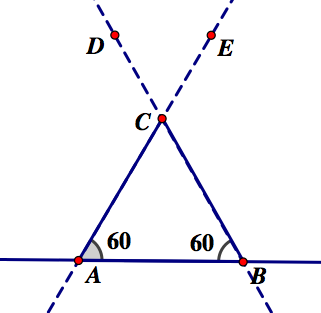
\includegraphics[width=2in]{4a.png}\end{center}
Note that $C\in H_E$ implies that $A,B,C$ are noncollinear so that we can consider triangle $\triangle ABC$. Also because $C\in H_E$ we know that $\ray{AC} = \ray{AE}$ and $\ray{BC}= \ray{BD}$, so that $$\angle BAE = \angle BAC \spand \angle ABD = \angle ABC.$$ By Theorem 5.1.3 the angle at vertex $C$ measures $180^\o - 60^\o - 60^\o = 60^\o.$ Therefore by Problem 3, $\triangle ABC$ is equilateral.\end{proof}

\item   (10 pts) Prove that if $\triangle ABC$ is an equilateral triangle, then the altitude through $A$, the median through $A$, and the perpendicular bisector of $\seg{BC}$ are the same line. 

\begin{proof} Let $D$ be the foot of the altitude from $A$ to $\line{BC}$. Note that since $A\notin\line{BC}$ we can refer to this altitude line as $\line{AD}$. Furthermore as we proved in the Lemma for Pointwise Characterization of Angle Bisectors, since angle $\angle BCA$ is acute by Problem 3, we know that $D\in \ray{CB}$. In the same way because $\angle CBA$ is acute, $D\in\ray{BC}$. Hence $D\in\seg{BC}$ and furthermore $B\ast D\ast C$, because if $D$ was a vertex of $\triangle ABC$ then one of the angles would measure $90^\o,$ contradicting Problem 3. Therefore $A,B,D$ and $A,C,D$ are each triplets of noncollinear points, so we can consider the triangles $\triangle ABD$ and $\triangle ACD$.

\begin{center}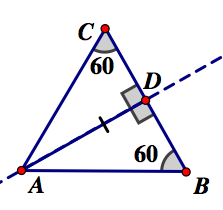
\includegraphics[width=2in]{5a.png}\end{center}

Since $$\angle ABD = \angle ABC \cong \angle ACB = \angle ACD$$ by Problem 3, $$\mu(\angle ADB) = \mu(\angle ADC) = 90^\o,$$ and $AD=AD,$ by AAS we have $\triangle ABD \cong \triangle ACD.$ Then $CD=DB$ and thus $D$ is the midpoint of $\seg{BC}$. It follows immediately that $\seg{AD}$ is the median through vertex $A$ and that $\line{AD}$ is the perpendicular bisector of segment $\seg{BC}$.
\end{proof}

\item (10 pts) Let $\triangle ABC$ be an equilateral triangle.  Prove that the orthocenter, $H$, the circumcenter $O$, and the centroid $G$ of $\triangle ABC$ coincide. 

\begin{proof} Let $\triangle ABC$ be an equilateral triangle. For each vertex $V$ of $\triangle ABC$, define $\ell_V$ to be the altitude line through $V$, $m_V$ to be the line containing the median through $V$, and $n_V$ to be the perpendicular bisector of the segment opposite $V$. Note that by definition (and existence by theorems in the Euclidean exploration), the orthocenter $H$, circumcenter $O$, and centroid $G$ of $\triangle ABC$ satisfy
$$\{H\} =\ell_A \cap \ell_B \cap \ell_C$$
$$\{ O\} = n_A \cap n_B \cap n_C$$
$$\{G \}= m_A \cap m_B \cap m_C.$$
Or, a bit pedantically, $\{G\}$ is the intersection of the medians, each of which are segments that are by definition subsets of the lines $m_V$, and therefore the intersection of the lines $m_V$ is $\{G\}$ as well. However because $\triangle ABC$ is equilateral, it is evident that the results of Problem 5 hold for each vertex of $\triangle ABC$. That is, for each vertex $V$ we have $\ell_V = n_V = m_V.$ It is then apparent from the three equalities above that $H=O=G.$\end{proof} 

\item  (10 pts) In a sort of converse to the previous problem, prove that if the circumcenter and the centroid  of a triangle $\triangle ABC$ coincide, then $\triangle ABC$ is equilateral.

\begin{proof} Let $\triangle ABC$ be a triangle and suppose the circumcenter $O$ and centroid $G$ of $\triangle ABC$ coincide. Define for each vertex $V$ the lines $\ell_V, m_V, n_V$ as in the previous problem, and let $D,E,$ and $F$ be the midpoints of the sides opposite the vertices $A,B,$ and $C$ respectively. Because $O=G$, the perpendicular bisector $n_A$ of side $\seg{BC}$ contains both the midpoint $D$ of $\seg{BC}$ and the centroid $G$. However by definition we know that $G\in m_A$, the median line through $A$. Thus
$$\{G,D\} \subseteq m_A \cap n_A,$$ and of course $G\ne D$ (certainly $D$ is not incident with all other medians), so it must be the case that $m_A=n_A$.
\begin{center}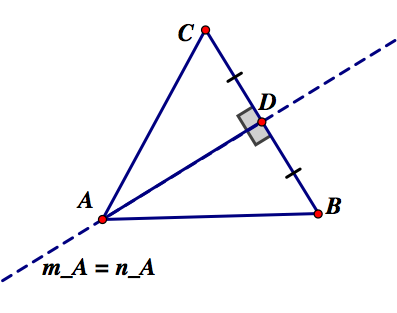
\includegraphics[width=3in]{7a.png}\end{center}
Therefore $m_A \perp \ \line{BC}$, so $\angle ADB$ and $\angle ADC$ are right angles. Also since $D$ is the midpoint of $\seg{BC}$ we have $BD=CD$, and of course $AD=AD$, so by SAS
$$\triangle ABD \cong \triangle ACD.$$
It follows that $\seg{AB}\cong\seg{AC}.$
\begin{center}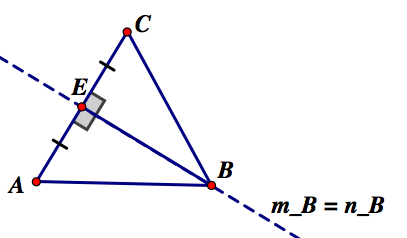
\includegraphics[width=3.3in]{7b.png}\end{center}
Of course considering vertex $B$ and applying the same argument will reveal that $m_B=n_B$, from which it follows that $\triangle BAE \cong \triangle BCE$, so that $\seg{AB}\cong\seg{BC}$. Therefore $\seg{AB}\cong \seg{BC}\cong\seg{AC}$, so $\triangle ABC$ is an equilateral triangle.\end{proof}

\item Let $O$ be a point and let $r > 0$.  Let $\cal C$ be the circle of radius $r$ centered at $O$. 
\begin{enumerate}
\item (10 pts) Prove that on any secant line $\ell$ there are points that lie inside $\cal C$ and there are points that lie outside $\cal C$. 

\begin{proof} Let $\ell$ be a secant line for $\C$ and $P,Q$ be the distinct points at which $\ell$ intersects $\C$. First we consider the case when $O\in\ell$. 
\begin{center}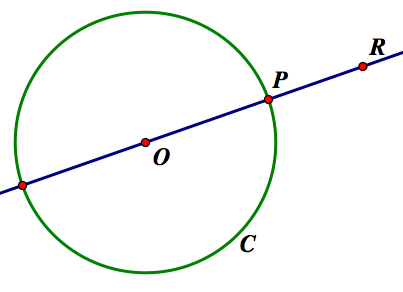
\includegraphics[width=3.3in]{8a1.png}\end{center}
Then half of the theorem is proven, and using the Ruler Postulate to pick a point $R$ on $\ray{OP}$ such that $OR>r$ shows that there exists $R\in\ell$ such that $R$ lies outside the circle.

Next suppose $O\notin\ell$. Let $R\in\ell$ such that $P\ast R\ast Q$.
\begin{center}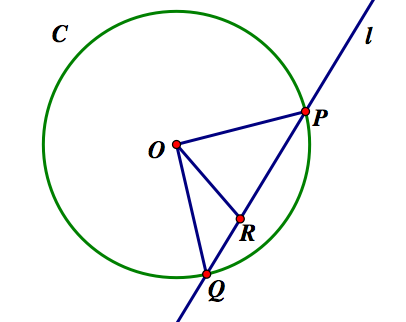
\includegraphics[width=3.3in]{8a2.png}\end{center}
Since $O\notin\ell,$ the angles $\angle QRO$ and $\angle ORP$ form a linear pair. It follows from the Linear Pair Theorem that at least one of them measures greater than or equal to $90^\o$. Without loss of generality we suppose that $\mu(\angle QRO) \ge 90^\o$. Then considering triangle $\triangle QRO$, the angles at the other vertices obviously measure less than $\angle QRO,$ so by the Scalene Inequality we have $OR<OQ=r$. Therefore $R$ lies inside $\C$. For a point outside $\C$, pick a point $S\in\ell$ such that $QS=2r$.
\begin{center}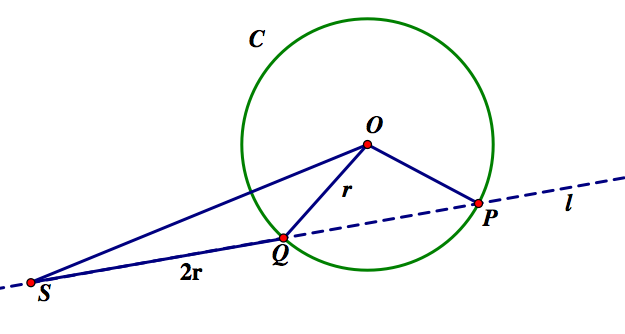
\includegraphics[width=3.8in]{8a3.png}\end{center}
Now since $Q,S,$ and $O$ are noncollinear, by the Triangle Inequality (Theorem 4.3.2) we have $QS < QO + OS,$ which means that $2r < r + OS$, and it follows that $OS>r$ so that $S$ lies outside of $\C$. Thus there exists points on $\ell$ that are inside $\C$ and points that are outside $\C$.\end{proof}

\item (10 pts) Prove that if $\ell$ is tangent to $\cal C$ at a point $Q$, then $OQ \perp \ell$. 

\begin{proof} Suppose $\ell$ is tangent to $\C$ at $Q$. First note that $O\notin\ell$, otherwise choosing $P\in\ell$ such that $P\ast O\ast Q$ and $PO=OQ$ reveals that $OP=OQ=r$, implying $P\in\C$ and contradicting $\ell$ tangent to $\C$.

Now suppose for contradiction that $\ell \not\perp \ \line{OQ}$. Then drop a perpendicular from $O$ to $\ell$ with foot $R$; note that by assumption $R\ne Q$. Now let $S\in\ell$ such that $Q\ast R\ast S$ and $QR=RS$; that is, such that $R$ is the midpoint of segment $\seg{QS}$.
\begin{center}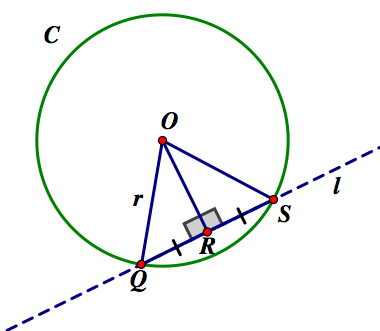
\includegraphics[width=3.3in]{8b1.png}\end{center}
Now we have $SR=QR$, angles $\angle QRO$ and $\angle SRO$ as congruent right angles, and $OR=OR$, so by SAS we conclude $\triangle QRO \cong \triangle SRO$. It follows that $OS=OQ=r$, implying that $S\in\C$ and contradicting $\ell$ tangent to $\C$. Therefore it must be the case that $\line{OQ} \ \perp\ell$.\end{proof}

\item (10 pts) Suppose that $\ell$ is tangent to $\cal C$ at $Q$.  Prove that every point on $\ell$ besides $Q$ lies outside the circle.  

\begin{proof} Let $P\in\ell\setminus\{Q\}$. As argued in part (b), $O\notin \ell$ so we can consider the triangle $\triangle OQP$.
\begin{center}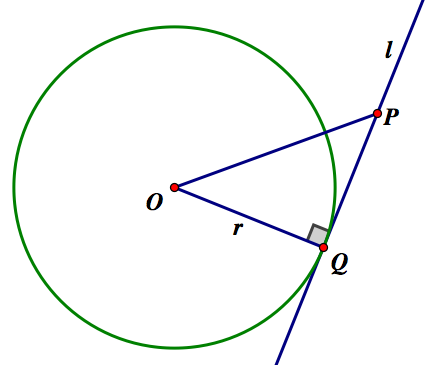
\includegraphics[width=3.3in]{8c.png}\end{center}
Since $\line{OQ}\perp\ell$ by part (b), we know that $\triangle OQP$ as a right angle at vertex $Q$. Hence by the Scalene Inequality, $OP>OQ=r$ so that $P$ lies outside of $\C$. This of course must hold for all such points $P\in \ell \setminus \{Q\}$.\end{proof}
\end{enumerate}

\item {\bf Asymptotic Pasch's Axiom?} Suppose that $\curlywedge DPAB$ is an asymptotic triangle and that $\ell$ is a line other than $\line{PD}$ or $\line{AB}$. Determine whether each statement is true or false.  Prove your answer. 

\begin{enumerate}
\item (10 pts) If $P \in \ell$, then $\ell \cap \ray{AB} \neq \emptyset$. 

\begin{proof} False! Construct $\ell$ as the double perpendicular line parallel to $\line{AB}$ through $P$; drop a perpendicular from $P$ to $\line{AB}$ with foot $F$ and let $\ell$ be the line perpendicular to $\line{PF}$ through $P$.
\begin{center}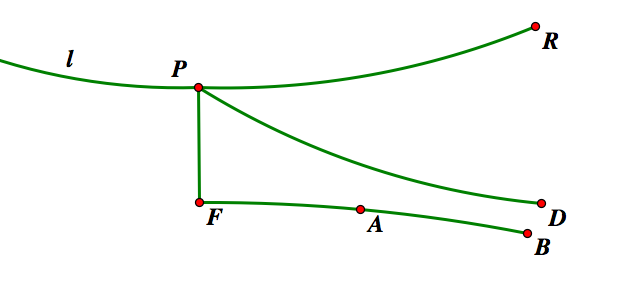
\includegraphics[width=4in]{9a.png}\end{center}
By endpoint independence we can possibly re-lable the point $B$ so that $\ray{PD} \ | \ \ray{FB}$. Choose a point $R\in\ell$ on the same side of $\line{PF}$ as $B$. The limiting parallel ray to $\ray{FB}$ through $P$ is uniquely $\ray{PD}$, and it cannot be the case that $\ray{PD}=\ray{PR}$ because the angle of parallelism $\angle FPD$ is acute by Theorem 6.3.8, whereas $\angle FPR$ is a right angle by construction. Therefore $\line{PD} \ \ne \ell$, and yet by construction $\ell \ \| \line{AB}$, so certainly  $\ell \cap \ray{AB} = \emptyset$. \end{proof}

\item (5 pts) If $A \in \ell$ and $E \in \ell$ such that $E$ is in the interior of $\angle BAP$, then $\ell \cap \ray{PD} \neq \emptyset$.  

\begin{proof} True! If $E$ is in the interior of $\angle BAP$, this means that ray $\ray{AE}$ is between the rays $\ray{AB}$ and $\ray{AP}$. Recall from symmetry of limiting parallelism that $\ray{PD} \ | \ \ray{AB}$ implies $\ray{AB} \ | \ \ray{PD}$. Thus since $\ray{AE}$ is between the rays $\ray{AB}$ and $\ray{AP}$, it must be the case that $\ray{AE}$ intersects $\ray{PD}$. Thus if both $A$ and $E$ lie on $\ell$, we have $\ell = \ \line{AE}$ from which it is clear that $\ell \cap \ray{PD} \ne \emptyset$.

\end{proof}

\item (10 pts) If $D \in \ell$, then $\ell \cap \ray{AB} \neq \emptyset$ or $\ell \cap \seg{PA} \neq \emptyset$.  

\begin{proof} True!

\begin{center}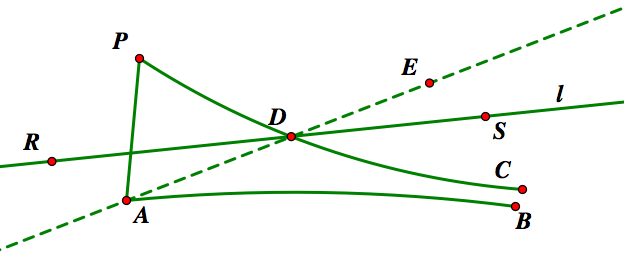
\includegraphics[width=4in]{9c.png}\end{center}
If $\ell = \ \line{DA}$ then $\ell\cap\ray{AB} = \{A\} \ne \emptyset$ and the proof is complete. So suppose $\ell \ne \line{DA}$ and choose $R,S\in\ell$ such that $R\ast D\ast S$, where $S$ is on the same side of $\line{DA}$ as $C$. Let $E$ be such that $A\ast D\ast E$ and let $C$ be such that $P\ast D\ast C$. By endpoint independence we have $\ray{DC} \ | \ \ray{AB}$. So if $\ray{DS}$ is between rays $\ray{DA}$ and $\ray{DC}$ then $\ray{DS} \cap \ray{AB} \ne \emptyset$, which of course implies $\ell \cap \ray{AB} \neq \emptyset$. If instead $\ray{DS}$ is not between $\ray{DA}$ and $\ray{DC}$, since $S$ and $C$ are on the same side of line $\line{DA}$, it follows from Lemma 3.4.4 that either $\ray{DC}=\ray{DS}$ or ray $\ray{DC}$ is between rays $\ray{DA}$ and $\ray{DS}$. Well $\ray{DC}=\ray{DS}$ implies that $\ell = \line{PD}$ which contradicts the hypothesis. So it must be the case that $\ray{DC}$ is between rays $\ray{DA}$ and $\ray{DS}$, and since $A\ast D\ast E$, we have from Lemma 3.5.7 that ray $\ray{DS}$ is between $\ray{DC}$ and $\ray{DE}$. Translating this into angle interiors, we have shown that $S$ is in the interior of angle $\angle EDC$, so that $S$ and  $E$ are on the same side of the line $\line{DC}=\line{PD}$. Since $A\ast D\ast E$ and $R\ast D\ast S$, it follows that $R$ and $A$ are on the same side of line $\line{PD}$. Similarly, since we chose $S,C$ on the same side of line $\line{DA}$, $P\ast D\ast C$ and $R\ast D\ast S$ implies that $P$ and $R$ are on the same side of line $\line{DA}$. This shows that $R$ is in the interior of $\angle PDA$. By the Crossbar Theorem, $\ray{DR}$ intersects the segment $\seg{PA}$, so we conclude $\ell \cap \seg{PA} \neq \emptyset$.  \end{proof}

\item (10 pts) If $\ell$ intersects the interior of $\seg{AP}$, then $\ell$ intersects either $\ray{PD}$ or $\ray{AB}$.  

\begin{proof} False! Let $E$ be any point in the interior of $\seg{AP}$, and note that $E\notin\line{AB}$. By Theorem 6.4.5 there is a unique ray $\ray{EF}$ such that $\ray{EF} \ | \ \ray{AB}$.

\begin{center}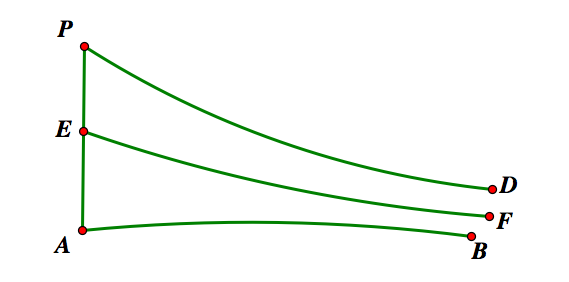
\includegraphics[width=4.1in]{9d.png}\end{center}
We also have $\ray{AB} \ | \ \ray{PD}$ by hypothesis, so by Theorem 6.4.7 either $\ray{EF} \ | \  \ray{PD}$ or $\ray{EF}$ is equivalent to $\ray{PD}$. However it is rather obvious that these rays are not equivalent. If $E\in\ray{PD}$ then since $E\ne P$ by construction, we would have $\ray{PD} = \ray{PE}$ which of course intersects $\ray{AB}$ at the point $A$ and is a contradiction. Thus $\ray{EF} \not\subseteq \ray{PD}$. Also if $P\in\ray{EF}$ then similarly we would have $\ray{EF}=\ray{EP}$. However from $A\ast E\ast P$ we see that this implies $\ray{EF}\subseteq\ray{AE}$, so that rays $\ray{EF}$ and $\ray{AE}$ are equivalent. But then from $\ray{EF} \ | \ \ray{AB}$, endpoint independence would imply that $\ray{AE} \ | \ \ray{AB}$, which is obviously a contradiction. Hence $ \ray{PD} \not\subseteq \ray{EF}$. Thus $\ray{EF}$ and $\ray{PD}$ are not equivalent rays and it follows from above that $\ray{EF} \ | \ \ray{PD}$. Therefore letting $\ell = \ \line{EF}$, we have from Theorem 6.4.2 that $$\ell \ \| \line{AB} \spand \ell \ \| \line{PD}.$$ So, we have found a line $\ell$ intersecting the interior of $\seg{AP}$ at a point $E$, and yet $\ell$ does not intersect the ray $\ray{PD}$ nor the ray $\ray{AB}$.
\end{proof}
\end{enumerate}

\end{enumerate}

\end{document}